\documentclass[letterpaper, reqno,11pt]{article}
\usepackage[margin=1.0in]{geometry}
\usepackage{color,latexsym,amsmath,amssymb,graphicx, float}
\usepackage{hyperref}

\hypersetup{
colorlinks=true,
linkcolor=magenta,
filecolor=magenta,
urlcolor=cyan,
}

\graphicspath{ {images/} }

\begin{document}
\pagenumbering{arabic}
\title{ELEC 481 Homework 5}
\date{04/06/22}
\author{Xander Naumenko}
\maketitle

{\noindent\bf Question 1a.} One method that one could use is contingent valuation. In this method you could ask people how much they would pay to reduce their commute by an hour, and this would give an estimate of the value. 

Another potential way to deduce the benefit would be the wages forgone method. By spending one extra hour one a commute people are sacrificing time that could be spent making money at the rate that one normally would, so a good baseline for the value of the saved hour would be one hours worth of wages. 

A method not suited for this situation is conjoint analysis, as the situation is quite simple and it is not a highly complex decision that people consider deeply. 

{\noindent\bf Question 1b.} One method that one could use is the hedonic price method. In this method you could look at the property value of places near nice bike paths and compare them to those near old unused railway tracks, and the difference between the two would signify the value people place on the construction of a new bike path. 

Another method you could use is again travel cost analysis. By seeing how much people pay/time people take to go to nice bike paths, you can get an idea of the benefit of constructing one. 

One valuation not necessarily suited for the situation is contingent valuation, as the presence of a bike path is public good that people aren't very good at valuating individually. 

{\noindent\bf Question 1c.} The first method that could be used to estimate the benefits of the project is measuring averting expenditures. For example people close to the river likely have precautions in place, and by looking at how much people spend on these precautions a monetary valuation can be deduced. 

Another way to consider the benefits would be replacement costs. If a flood did occur you could measure the hypothetical total costs of the disaster (including lives/injuries), and a reduction of this happening by 5\% chance would be the benefit associated with the project. 

One method that wouldn't work well for this situation is travel cost method. Since the project isn't constructing anything that could be construed as a destination it wouldn't make sense to see how much people would pay to see the improvement. 

{\noindent\bf Question 1d.} Perhaps the best method to evaluate the benefit of this project is the travel cost method. People routinely spend lots of money going to national parks, so by looking at how much people spend an evaluation of the benefits can be attained. 

Another method that could be used is the averting expenditures methods. By seeing how much more people pay to go to national parks relative to the next best option, this would give an idea as to the benefit of the project. 

A method not suited for this situation would be the wages forgone method. Since this isn't a hazard-based project and is instead large scale public planning it doesn't make sense to think about. 

{\noindent\bf Question 1e.} One way to measure this is the wages forgone method. People often work riskier jobs for a chance of higher pay, so by seeing how much pay people are willing to sacrifice for a safer job the value that people place on their own lives can be obtained. 

Another way to think about the value of a human life is averting behavior. People will expend money to avoid being in risky situations, and the amount that they pay (adjusted for the increase in risk) gives the value they place on a life. 

A valuation method not suited for this is replacement cost. Clearly a human life can't simply be replaced, so no monetary value for such a thing could be obtained. 

{\noindent\bf Question 2a.} Clearly with $\$200000$ two of the projects will be selected. Because all the capital costs are the same, the best two projects will be those with the highest IRRs (this is only valid since their capital costs are the same). Putting the given values into excel as seen in figure \ref{fig:q2} and using the builtin IRR function, we find: 

\begin{figure}[htpb]
    \centering
    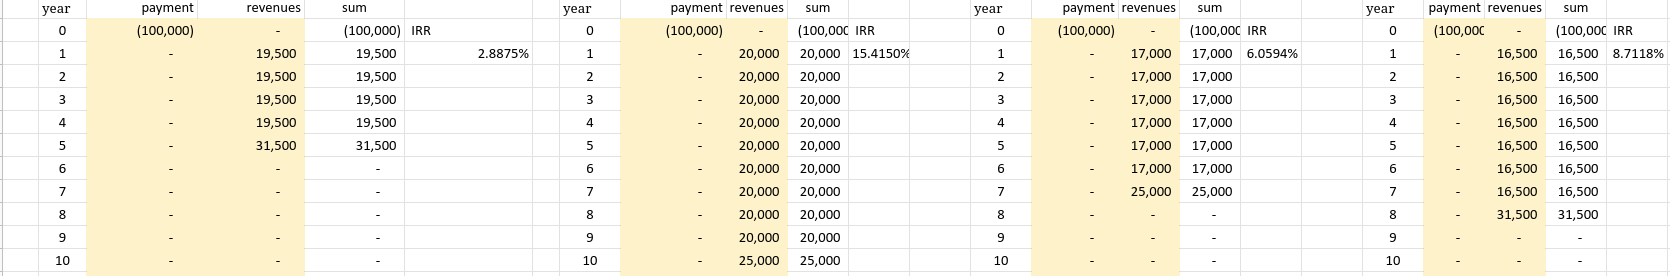
\includegraphics[width=0.8\textwidth]{q2}
    \caption{Revenue flow for question 2}
    \label{fig:q2}
\end{figure}

 \[
IRR_A = 2.9\%
.\]
 \[
IRR_B = 15.4\%
.\]
 \[
IRR_C = 6.1\%
.\]
 \[
IRR_D = 8.7\%
.\]

Because option B and D have the highest rate of return they are the investements that should be chosen. 

{\noindent\bf Question 2b.} The opportunity cost of capital is the return of next best option, which in this case is option C with 6.1\%. 

{\noindent\bf Question 3a.} See the table in figure \ref{fig:q3}. The IRR for each is computed and used to rank the options. Luckily the three best options, options 1, 6 and 7, sum to exactly \$70000 so that's what should be chosen. 
\begin{figure}[htpb]
    \centering
    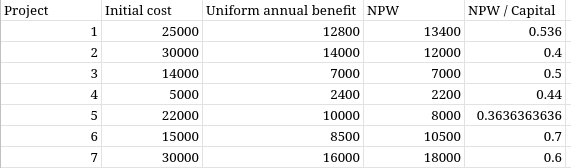
\includegraphics[width=0.8\textwidth]{q3}
    \caption{Analysis of each option for question 3}
    \label{fig:q3}
\end{figure}

{\noindent\bf Question 3b.} The opportunity cost of capital is the benefit of the next best option, so in this case it would be a rate of return of \%23.4. 

{\noindent\bf Question 4a.} Since options E and G have a lower computed rate of return than the MARR, they shouldn't be considered. All other options should still be considered further. 

{\noindent\bf Question 4b.} See figure \ref{fig:q4}. It is calculated in excel and has all the required values. 

\begin{figure}[htpb]
    \centering
    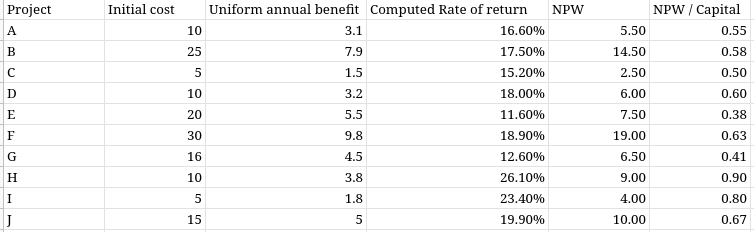
\includegraphics[width=0.8\textwidth]{q4}
    \caption{Computed values for question 4b}
    \label{fig:q4}
\end{figure}

{\noindent\bf Question 4c.} Based on figure \ref{fig:q4}, wee see that the order of the most desirable (i.e. highest NPW / PW) is H, I, J, F, D, B, A, C, G and then E. 

{\noindent\bf Question 4d.} Going down the list in the order listed in the previous part and each time getting the next cheapest projects, we should approve projects H, I, J, F, D and A and C. 

\end{document}
